% -----------------------------------------------
% Template for ISMIR Papers
% 2016 version, based on previous ISMIR templates

% Requirements :
% * 6+1 page length maximum
% * 2MB maximum file size
% * Copyright note must appear in the bottom left corner of first page
% (see conference website for additional details)
% -----------------------------------------------

\documentclass{article}
\usepackage{ismir,amsmath,cite}
\usepackage{graphicx}
\usepackage{color}
\usepackage[]{algorithm2e}
\usepackage{color}
\usepackage{multirow}
\usepackage{subfigure}
\usepackage[justification=centering]{caption}
\usepackage{epstopdf}
\usepackage{float} 
\usepackage{amssymb}
\usepackage[]{algorithm2e}
\usepackage{enumitem} 
%\sloppy


% Title.
% ------
\title{Genre specific dictionaries for harmonic/percussive source separation}

% Note: Please do NOT use \thanks or a \footnote in any of the author markup

% Single address
% To use with only one author or several with the same address
% ---------------
%\oneauthor
% {Names should be omitted for double-blind reviewing}
% {Affiliations should be omitted for double-blind reviewing}

% Two addresses
% --------------
%\twoauthors
%  {First author} {School \\ Department}
%  {Second author} {Company \\ Address}

% Three addresses
% --------------
%\threeauthors
%  {First author} {Affiliation1 \\ {\tt author1@ismir.edu}}
%  {Second author} {\bf Retain these fake authors in\\\bf submission to preserve the formatting}
%  {Third author} {Affiliation3 \\ {\tt author3@ismir.edu}}

% Four addresses
% --------------
\fourauthors
  {First author} {Affiliation1 \\ {\tt author1@ismir.edu}}
  {Second author}{Affiliation2 \\ {\tt author2@ismir.edu}}
  {Third author} {Affiliation3 \\ {\tt author3@ismir.edu}}
  {Fourth author} {Affiliation4 \\ {\tt author4@ismir.edu}}

\begin{document}
%
\maketitle
%


\begin{abstract}

Blind source separation usually obtains limited performance on real and polyphonic music signals. To overcome these limitations, it is common to rely on prior knowledge under the form of side information as in Informed Source Separation or on machine learning paradigms applied on a training database. In the context of source separation based on factorization models such as the Non-negative Matrix Factorization, this supervision can be introduced by learning specific dictionaries. However, due to the large diversity of musical signals it is not easy to build sufficiently compact and precise dictionaries that will well characterize the large array of audio sources. In this paper, we argue that it is relevant to construct genre-specific dictionaries. Indeed, we show on a task of harmonic/percussive source separation that the dictionaries built on genre-specific training subsets allow to reach a better performance than cross-genre dictionaries.



\end{abstract}
%
\section{Introduction}\label{sec:introduction}


\emph{Source separation} is a field of research that seeks to separate the components of a recorded audio signal. Such a separation has many applications in music such as up-mixing \cite{fitzgerald2011upmixing} (spatialization of the sources) or automatic transcription \cite{vincent2010adaptive} (it is easier to work on single sources). The separation task is difficult due to the complexity and the variability of the music mixtures. 


The large variety of audio signals can be classified into various musical genres \cite{tzanetakis2002musical}. Genres are labels created and used by humans for categorizing and describing music. They have no strict definitions and boundaries but particular genre share certain characteristics typically related to instrumentation, rhythmic structure, and pitch content of the music. This resemblance between two pieces of music has been used as an information to improve chord transcription \cite{ni2012using,lee2008acoustic} or downbeat detection \cite{hockman2012one} algorithms. Genre information can be obtained using annotated labels. When the genre information is not available, it can be retrieved using automatic genre classification algorithms \cite{tzanetakis2002musical,mckay2006musical}. Such classification have never been used to guide a source separation problem. Furthermore, most datasets used for Blind Audio Source Separation (BASS) research are small in size and they do not allow for a thorough comparison of the source separation algorithms. Using a larger database is crucial to benchmark the different algorithms.

In the context of BASS, Non-negative Matrix Factorization (NMF) is a widely used method. The goal of NMF is to approximate a data matrix $V \in \mathbb{R}_{+}^{n \times m} $ as 
\begin{equation}\label{modelNMF}
V \approx \tilde{V} = WH
\end{equation}
with $W \in \mathbb{R}_{+}^{n \times k}$, $H \in \mathbb{R}_{+}^{k \times m}$ and where $k$ is the rank of factorization \cite{lee99}. In audio signal processing, the input data is usually a Time-Frequency (TF) representation such as a STFT or a constant-Q transform spectrogram. Blind source separation is a difficult problem and the plain NMF decomposition does not provide satisfying results. To obtain a satisfying decomposition, it is necessary to exploit various features that make each source distinguishable from one another. 
Supervised algorithms in the NMF framework exploit training data or prior information in order to guide the decomposition process. For example, information from the scores or from midi signals can be used to initialize the learning process \cite{EwertM12}. The downside of these approaches is that they require well organized prior information that is not always available. Another supervised method consists in performing prior training on specific databases. A dictionary matrix $W_{train}$ can be learned from database in order to separate instruments \cite{jaureguiberry2011adaptation,wudrum}. Such methods require minimum tuning from the user.  However, within different music pieces of an evaluation database, the same instrument can sound differently depending on the recording conditions and post processing treatments. In order to accurately represent an instrument, one can decide to learn a dictionary on a very large database but takes the risk of over-fitting the data.% The dictionaries must match the target instruments to obtain satisfying performances. 


In this paper, we focus on the task of Harmonic/Percussive Source Separation (HPSS). HPSS has numerous applications as a preprocessing step for other audio tasks. For example the HPSS algorithm~\cite{fitzgerald2010harmonic} can be used as a preprocessing step to increase the performance for singing pitch extraction and voice separation~\cite{hsu2012tandem}. 
%most multi-pitch estimation models~\cite{klapuri2008multipitch}, instruments recognition~\cite{eronen2000musical} and melody extraction~\cite{salamon2012melody} algorithms are much more efficient when processing harmonic data only. 
Similarly, beat tracking~\cite{ellis2007beat} and drum transcription algorithms~\cite{paulus2005drum} are more accurate if the harmonic instruments are not part of the analysed signal. 

We built our algorithm using the method developed in \cite{laroche2015structuredhidden}: an unconstrained NMF decomposes the audio signal in sparse orthogonal components that are well suited for representing the harmonic component, while the percussive part is represented by a regular nonnegative matrix factorization decomposition. In \cite{larocheJournalhidden}, we have adapted the algorithm using a trained drum dictionary to improve the extraction of the percussive instruments. As the databases cover a wide variety of genres, instrumentation may strongly differ from one piece to another. In order to better manage the variability and to build effective dictionaries, we propose now to use genre specific training data.

The main contribution is that we develop a genre specific method to build NMF drum dictionaries that give consistent and robust results on a HPSS task. The \emph{genre specific dictionaries} are able to improve the separation score compared to a \emph{universal dictionary} trained from all available data (i.e. a cross-genre dictionary). 


The rest of the paper is organized as follow. Section \ref{defgenre} defines the context of our work, Section \ref{sec:SPNMF} presents the proposed algorithm while Section \ref{ConstrucDict} describes the construction of specific dictionaries. Finally Section \ref{sec:results} details the results of the HPSS on $65$ audio files and  we suggest some conclusions in Section \ref{sec:conclusion}. 



\section{Toward genre specific information}\label{defgenre}

\subsection{Genre information}

Musical genre is one of the most prominent high level music descriptors. Electronic Music Distribution has become more and more popular in recent years and music catalogues never stop to increase (the biggest online services now propose around 1 million tracks). In that context, associating a genre to a musical piece is crucial to help users finding what they are looking for. As mentioned in the introduction, genre information has been used as a cue to improve some content-based music information retrieval algorithms. If an explicit definition of musical genres is not really available \cite{aucouturier2003representing}, musical genre classification can be performed automatically \cite{li2003comparative}. %{\color{red}{HP : il manque quelque chose ou enlever ``using different set of features''}}.

%Source separation has been used extensively in order to help the genre classification process \cite{rump2010autoregressive,lampropoulos2005musical}. However, genre information has not been yet exploited to guide the decomposition process. 
Source separation has been used extensively in order to help the genre classification process \cite{rump2010autoregressive,lampropoulos2005musical} but, as far as we know, it is the first time that the genre information is exploited to guide the decomposition process. 


\subsection{Methods for dictionary learning}

%{\color{red}{HP: la progression n'est pas tres claire. Mieux expliquer pourquoi on cherche a apprendre des dictionnaires. Comment et ou sont-ils utilises? Les idees sont la mais c'est un peu confus.}}  

Audio data is largely redundant as it often contains multiple correlated versions of the same physical event (note, drum hits...) \cite{tovsic2011dictionary}. The relevant information is generally of much reduced dimensionality compared to the original data sets hence the idea to exploit this redundancy to reduce the amount of information necessary for the representation of a musical signal. 

Many rank reduction methods, such as Single Value Decomposition (K-SVD)~\cite{aharon2006img}, Vector Quantization (VQ)~\cite{gersho2012vector}, Principal Component Analysis (PCA)~\cite{huang2012singing}, or Non negative matrix factorization (NMF)~\cite{Smaragdis03} are based on the principle that our observations can be described by a sparse subset of atoms taken from a redundant representation. These methods provide a small subset of relevant templates that are later used to guide the extraction of a target instrument. 

%{\color{red}{repetition!}} to use these methods to create genre specific drum dictionaries. {\color{red}{HP: c'est ici qu'il faut retravailler}}

Building a dictionary using K-SVD has been a successful approach in image processing applications\cite{zhang2010discriminative}. However this method does not scale well to process large audio signals as the computational is unrealistic. Thus a genre specific dictionary cannot be considered in this framework.

VQ has been mainly used for audio compression \cite{gersho2012vector} and PCA has been used for voice extraction \cite{huang2012singing}. However these methods do not have been used yet has a pre-processing step to build a dictionary. 
%, sparse coding has been used among other things for source separation \cite{plumbley2010sparse} 

Finally, in the NMF framework, some work has been done to perform a decomposition with learned dictionaries. In \cite{hennequin2011score}, the dictionary is built using a physical model of the instrument. This method is not adapted to build genre specific data as the model cannot easily take into account the genre information. 
A second way to build the dictionary is to directly use the Short Time Fourier Transform (STFT) of an instrument signal~\cite{wudrum}. This method does not scale well if the training data are large so it is not possible to use it to build genre specific information. 
Finally, another method using NMF to build a dictionary is to compute a NMF decomposition on a large training set specific to the target source \cite{schmidt2006single}. After the optimization process of the NMF, the $W$ matrix from this decomposition is used as the dictionary matrix $W_{train}$. This method is difficult to use on pitched instruments (i.e., harmonic instruments) and the dictionary needs to be adaptated using linear filtering on the fixed templates \cite{jaureguiberry2011adaptation}. If the fixed dictionaries provide good results for HPSS \cite{larocheJournalhidden}, the results have a high variance because the dictionary are learned on general data that do not take into account the large variability of drum sounds. Finally, the rank of the factorization determines the final size of the dictionary and it can be chosen small enough to obtain a strong compression of the original data. These properties motivated us to build genre specific data using NMF in order to obtain relevant compact dictionaries. 


%{\color{red}{HP: Bons resultats sur HPSS et ca nous motive pour le genre specifique??? le lien logique nest pas clairÉ }}. The selection of the rank of factorization will be discussed in Section \ref{optimalsize} {\color{red}{HP: chest etrange d'en parler ici. Ou aloes avannt il taut dire que c'est reste un problems ouvert}}.  

\subsection{Genre information for HPSS}

Current state-of-the-art unsupervised methods for HPSS such as \cite{ono2008separation} and \cite{canadas2014percussive} cannot be easily adapted to use genre information. In~\cite{kim2011nonnegative} the drum source separation is done using a Non-Negative Matrix Partial Co-Factorization (NMPCF). The spectrogram of the signal and the drum-only data (obtained from prior learning) are simultaneously decomposed in order to determine common basis vectors that capture the spectral and temporal characteristics of the drum sources. The percussive part of the decomposition is constrained while the harmonic part is completely unconstrained. As a result, the harmonic part 
tends to decompose a lot of information from the signal and the decomposition is not satisfactory (i.e., the harmonic part contains some percussive instruments). Another drawback of this method is that it does not scale when the training data is large and the computation time is significantly larger compared to other methods.

% Finally the method first introduced by \cite{laroche2015structuredhidden} and detailed in \cite{larocheJournalhidden} is a good candidate to test the genre specific dictionaries as they are easily integrated to the algorithm and do not increase the computation time. The method is briefly reminded in Next Section.

Next Section gives a short reminded of the approach introduced and detailled in~\cite{laroche2015structuredhidden,larocheJournalhidden} which appears to be a good candidate to test the genre specific dictionaries: they can be easily integrated to the algorithm without increasing the computation time. %The method is briefly reminded in Next Section.



\section{Structured projective NMF (SPNMF)}
\label{sec:SPNMF}

%In this section we present our algorithm for harmonic/percussive source separation.


\subsection{Principle of the SPNMF}

Using a similar model as in our preliminary work~\cite{laroche2015structuredhidden}, let $V$ be the magnitude spectrogram of the input data. The model is then given by
\begin{equation} \label{Cfunction}
V \approx \tilde{V}= V_H + V_{P},
\end{equation}
with $V_P$ the spectrogram of the percussive part and $V_H$ the spectrogram of the harmonic part. $V_H$ is approximated by the projective NMF decomposition \cite{yuanOja2005} while $V_P$ is decomposed by NMF components which leads to:
\begin{equation}
V \approx \tilde{V}= W_{H}W_{H}^{T}V + W_{P} H_{P}.
\end{equation}
The data matrix is approximated by an almost orthogonal sparse part that codes the harmonic instruments $V_H = W_HW_H^T V$ and a non constrained NMF part that codes the percussive instruments $V_P = W_PH_P$. As a fully unsupervised SPNMF model does not allow for a satisfying harmonic/percussive source separation~\cite{laroche2015structuredhidden}, we propose here to use a fixed genre specific drum dictionary $W_P$ in the percussive part of the SPNMF.



\subsection{Algorithm Optimization}

In order to obtain such a decomposition, we can use a measure of fit $D(x|y)$ between the data matrix $V$ and the estimated matrix $\tilde{V}$. $D(x|y)$ is a scalar cost function and in this article, we use the Itakura Saito (IS) divergence. A discussion about the possible use of other divergences can be found in \cite{larocheJournalhidden}.

The SPNMF model gives the optimization problem : 
\begin{equation}\label{InitCost}
\min_{W_H,W_P,H_P \geq 0} D(V|W_{H}W_{H}^{T}V + W_{P} H_{P})  
\end{equation}

A solution to this problem can be obtained by iterative multiplicative update rules following the same strategy as in~\cite{yuanOja2005,Lee01algorithmsfor} which consists in splitting the gradient with respect to (wrt) one variable (here $W_H$ for example) $\nabla_{W_H} D(V|\tilde{V})$ in its positive $[\nabla_{W_H} D(V|\tilde{V})]^{+}$ and negative parts $[\nabla_{W_H} D(V|\tilde{V})]^{-}$, if $\otimes$ is the Hadamard product or element-wise product. Using formula from Appendix~\ref{ISdisteq}, the SPNMF optimization process is given in Algorithm~\ref{AlgoDictionary}.
 
\begin{algorithm}[h]
 Input: $V \in \mathbb{R}_{+}^{m \times n} $
 Output: $W \in \mathbb{R}_{+}^{m \times k}$, $W_{train} \in \mathbb{R}_+^{m \times e}$ and $H \in \mathbb{R}_{+}^{e \times n}$
 Initialization\;
 \While{$i \leq$ number of iterations}{
	$H_{P} \leftarrow H_{P} \otimes \frac{ [\nabla_{H_P} D(V|\tilde{V})]^{-} }{[\nabla_{H_P} D(V|\tilde{V})]^{+}}$
	

	$W_{H} \leftarrow W_{H} \otimes \frac{ [\nabla_{W_H} D(V|\tilde{V})]^{-} }{[\nabla_{W_H} D(V|\tilde{V})]^{+}}$
	 \vspace{0.2cm}
	 	
	$i=i+1$ 
 }
 $ X_P = W_{train}H_P $ and
 $ X_H = W_HW_H^TV $ 
  
\vspace{0.2cm}
 \caption{SPNMF with a fixed trained drum dictionary matrix.}\label{AlgoDictionary}
\end{algorithm}




 
\subsection{Signal reconstruction}

The percussive signal $x_p(t)$ is synthesized using the magnitude percussive spectrogram $X_P = W_PH_P$. To reconstruct the phase of the percussive part, we use a Wiener filter~\cite{liutkus2015generalized} to create a percussive mask as:
\begin{equation}
\mathcal{M}_P = \frac{X_P^2}{X_M^2 + X_P^2}
\end{equation} 
To retrieve the percussive signal as, 
\begin{equation}
x_p(t) = InverseSTFT(\mathcal{M}_P \otimes X).
\end{equation}
Where $X$ is the complex spectrogram of the mixture.
We use a similar process for the harmonic part.
%, we obtain:
%\begin{equation}\label{percuweiner}
%\mathcal{M}_H = \frac{X_H^2}{X_M^2 + X_P^2},
%\end{equation}
%and:
%\begin{equation}
%x_h(t) = InverseSTFT(\mathcal{M}_H \otimes X).
%\end{equation}
%




\section{Construction of the dictionary}\label{ConstrucDict}

%In this Section, we present in Section \ref{optimalsize} the test conducted on the SiSEC $2010$ database~\cite{SiSec10} in order to find the optimal size to build the genre specific dictionaries. In Section \ref{database} we describe the training and the evaluation database. Finally, in Section \ref{genrespecdict}, we detail the protocol to build the genre specific dictionaries. 
In this section we detail the building process of the dictionary. We present in Section \ref{optimalsize} the test conducted on the SiSEC $2010$ database~\cite{SiSec10} in order to find the optimal size to build the genre specific dictionaries. In Section \ref{database} we describe the training and the evaluation database. Finally, in Section \ref{genrespecdict}, we detail the protocol to build the genre specific dictionaries. 

\subsection{Optimal size for the dictionary}\label{optimalsize}

The first step to build a NMF drum dictionary is to select the rank of factorization. In order to avoid overtraining, the algorithm is optimized using databases different from the database used for evaluation, described in Section \label{database}. 

We run the optimization tests on the public SiSec database from~\cite{SiSec10}. The database is composed of four polyphonic real-world music excerpts and each music signal contains percussive, harmonic instruments and vocals. The duration of the recordings is ranging from $14$ to $24$~s. In the context of HPSS, following the same protocol as in~\cite{canadas2014percussive}, we do not consider the vocal part and we build the mixture signals from the percussive and harmonic instruments only. The signals are sampled at $44.1$ kHz. We compute the STFT with a $2048$ sample long Hann window with a $50\%$ overlap. Furthermore, the rank of factorization of the harmonic part of the SPNMF algorithm is set to $k=100$, as in \cite{larocheJournalhidden}.

A fixed drum dictionary is built using the database ENST-Drums \cite{gillet2006enst}. For this, we  concatenate $30$ files were the drummer is playing a \emph{drum phrase} that result in an excerpt of around $10$~min duration. We then compute an NMF decomposition with different ranks of factorization ($k=12$, $k=50$, $k=100$, $k=200$, $k=300$, $k=500$, $k=1000$ and $k=2000$) on the drum signal alone to obtain $8$ drum dictionaries.

These dictionaries are then used to perform a HPSS on the four songs of the SiSEC database using the SPNMF algorithm. The results are compared by means of the Signal-to-Distortion Ratio (SDR), the Signal-to-Interference Ratio (SIR) and the Signal-to-Artifact Ratio (SAR) of each of the separated sources using the BSS Eval toolbox provided in \cite{bsseval}.

\begin{figure}[h]

  \centering 
  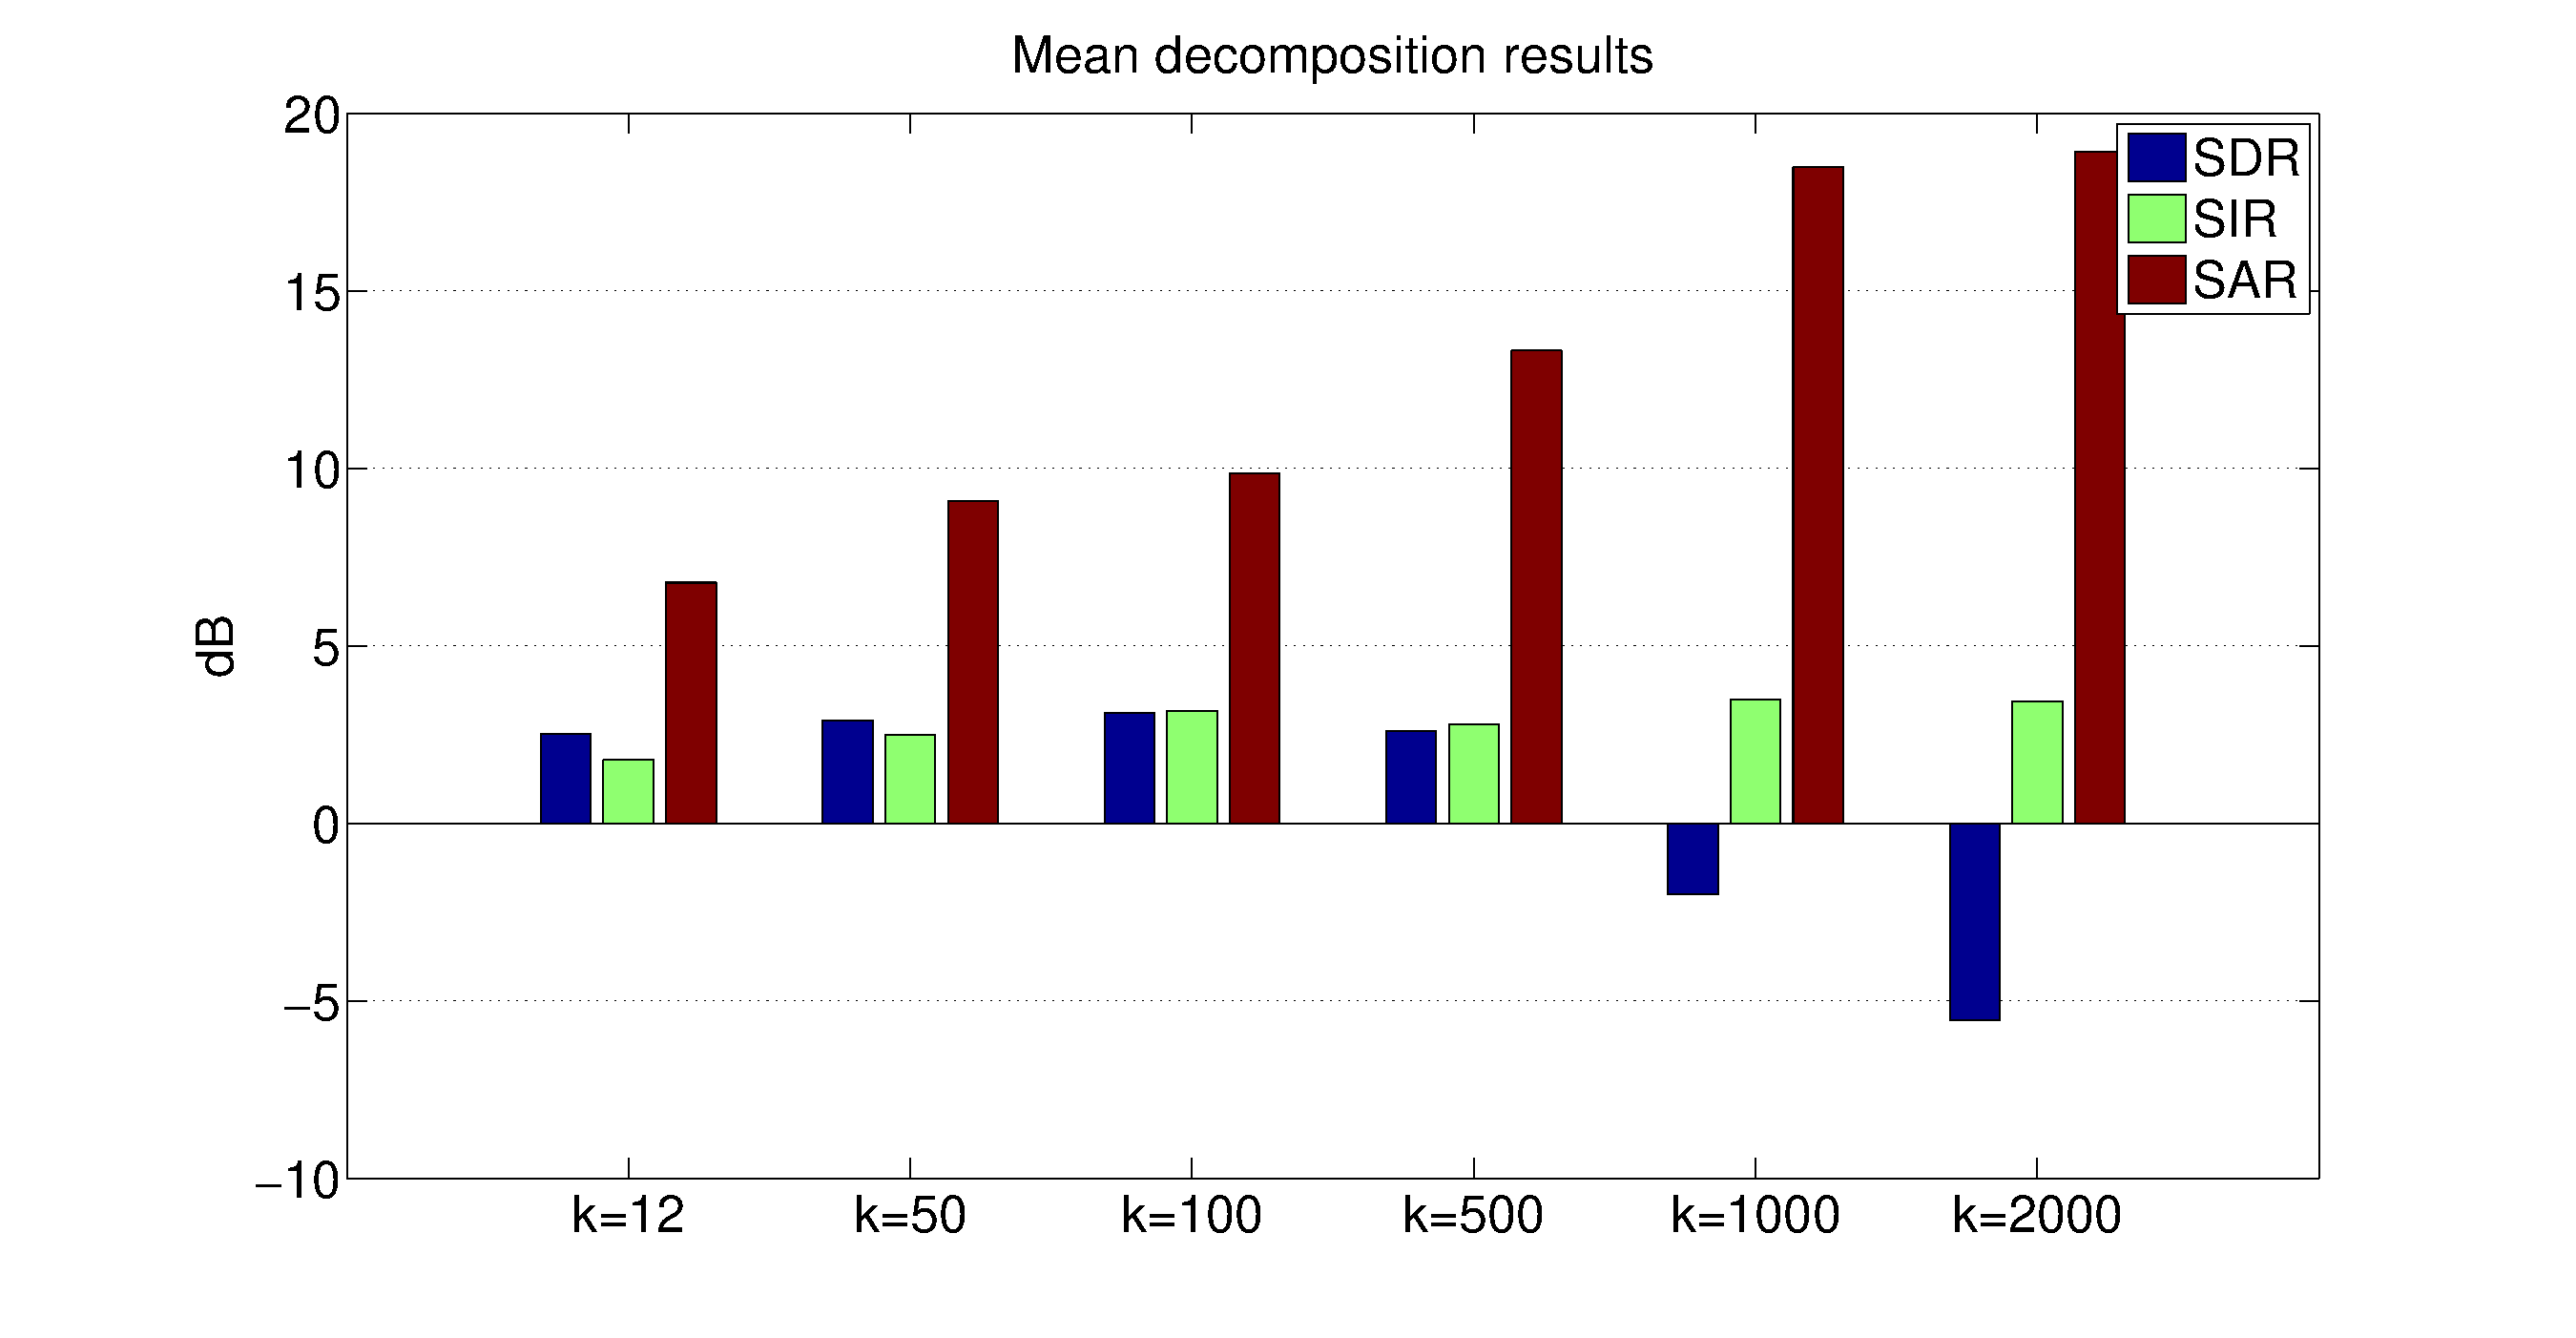
\includegraphics[width=9cm]{figs/AllDictSizeISMIR.eps}
%  \vspace{2.0cm}
  \caption{\label{dictsize}Influence of k on the S(D/I/A)R on the SiSEC database.}
  
\end{figure}

The results in Figure \ref{dictsize} show that the optimal value for the SDR and SIR is reached for $k=100$, then the SDR decreases for $k\geqslant 200$. The high values of SAR (for $k\geqslant 500$) are explained by the fact that the separation process is not satisfying. The harmonic signal provided by the algorithm contains most of the original signal therefore the SAR is very high but the decomposition quality is poor. For the rest of the article, the size of the drum dictionaries will be $k=100$.
%\textcolor{red}{The optimal dictionary size for the SPNMF algorithm is $k=100$ so we will use it in the next Section. $k=50$ and $k=200$ does not lead to significantly different. The method is robust and the to the rank of factorization.}

\subsection{Training and evaluation database}\label{database}

The evaluation test are conducted on the Medley-dB database \cite{bittner2014medleydb} composed of polyphonic real-world music excerpts. It has $122$ music signals and $85$ of them contain percussive instruments, harmonic instruments and vocals. The signals that do not contain a percussive part are excluded from evaluation. The genres are distributed as follows: \emph{Classical} ($8$ songs), \emph{Singer/Songwriter} ($17$ songs), \emph{Pop} ($10$ songs), \emph{Rock} ($20$ songs), \emph{Jazz} ($11$ songs), \emph{Electronic/Fusion} ($13$ songs) and \emph{World/Folk} ($6$ songs). Because the notion of genre is quite subjective (see Section \ref{defgenre}), the Medley-dB database uses general genre labels that cannot be considered to be precise. There are many instances where a song could have fallen in multiple genres, and the choices were made so that each genre would be as acoustically homogeneous as possible. Moreover, as we are only working with the instrumental part of the song (the vocals are omitted), the \emph{Pop} label (for example) are similar to the \emph{Singer/Songwriter}. We separate the database into training and evaluation files. 

\begin{table} 
	\centering 
	\small
   \begin{tabular}{|l|l|}
   \hline
   Genre & Artist Song \\
   	\hline   
Classical  & JoelHelander Definition \\
 & MatthewEntwistle AnEveningWithOliver \\
 & MusicDelta Beethoven \\
\hline
Electronic/Fusion & EthanHein 1930sSynthAndUprightBass \\
 & TablaBreakbeatScience Animoog \\
 & TablaBreakbeatScience Scorpio \\
\hline
Jazz & CroqueMadame Oil \\
 & MusicDelta BebopJazz \\
 & MusicDelta ModalJazz \\
\hline
Pop &  DreamersOfTheGhetto HeavyLove \\
 & NightPanther Fire \\
 & StrandOfOaks Spacestation \\
\hline
Rock & BigTroubles Phantom \\
 & Meaxic TakeAStep \\
 & PurlingHiss Lolita \\
\hline
Singer/Songwriter	& AimeeNorwich Child \\
 & ClaraBerryAndWooldog Boys \\
 & InvisibleFamiliars DisturbingWildlife \\
\hline
World/Folk & AimeeNorwich Flying \\
 &KarimDouaidy Hopscotch \\
 & MusicDelta ChineseYaoZu\\
\hline
Non specific & JoelHelander Definition \\
 & TablaBreakbeatScience Animoog \\
 & MusicDelta BebopJazz \\
 & DreamersOfTheGhetto HeavyLove \\
 &  BigTroubles Phantom \\
 & AimeeNorwich Flying \\
 &  MusicDelta ChineseYaoZu\\
 \hline

  
\end{tabular} 
\caption{\label{trainingdata} Song selected for the training database.}

\end{table}





\subsection{Genre specific dictionaries}\label{genrespecdict}

Seven genre-specific drum dictionaries are built using $3$ songs of each genre. In addition, a cross-genre drum dictionary is built using half of one song of each genre. Finally, a dictionary is built using the $10$~min excerpt of pure drum signals from the ENST-Drums database described in Section \ref{optimalsize}. The Medley-dB files selected for training are given in Table \ref{trainingdata} and excluded from evaluation. 

The NMF model is given by \eqref{modelNMF}. If $V$ is the power spectrum of a drum signal, The matrix $W$ is a {\em dictionary} or a set of {\em patterns} that codes the frequency information of the drum. Here we build genre specific drum dictionaries using the medley-dB database. %Using dictionaries specific to the genre of music allows to have dictionaries that a more specific to the signal to decompose.

%Table \ref{lengthDict} gives us the length and the energy of the training signal for each genre.
%\emph{Classical} and \emph{Electronic/Fusion} songs are composed of songs where the drum is only playing for a few moments and even though the signals are longer than the other. 
With the results from Section \ref{optimalsize} the dictionaries are built as follows: for every genre specific subset of the training database, we perform a NMF on the drum signals with $k=100$,  the $W$ matrices of the NMF are then used in the SPNMF algorithm as the  $W_P$ matrix (see Algorithm \ref{AlgoDictionary}).

%\begin{table}
%   
%	\centering 
%   \begin{tabular}{|l|l|}
%\hline   
%Genre & Length(min) \\
%\hline
%Classical  & 22.06  \\
%\hline
%Electronic/Fusion & 18.66 \\
%\hline
%Jazz & 10.96 \\
%\hline
%Pop &  12.53 \\
%\hline
%Rock & 11.43 \\
%\hline
%Singer/Songwriter & 9.36 \\
%\hline
%World/Folk & 9.53 \\
%\hline
%Non Specific (Mix) & 11.03  \\
%\hline
%  
%\end{tabular} 
%\caption{\label{lengthDict} Length of the genre specific database.}
%\end{table}


\section{Results}\label{sec:results}

In this Section, we present the results of the SPNMF with the genre specific dictionaries on the evaluation database from Medley-dB.

\subsection{Comparison of the dictionaries}

We perform a HPSS on the audio files using the SPNMF with the $9$ dictionaries build in Section \ref{genrespecdict}. The results on each song are then sorted by genres and the average results are displayed using box-plots. Each box-plot is made up of a central line indicating the median of the data, upper and lower box edges indicating the $1^{st}$ and $3^{rd}$ quartiles while the whiskers indicate the minimum and maximum values. 


The Figures \ref{sdrpop}, \ref{sirpop} and \ref{sarpop} show the SDR, SAR and SIR results for all the dictionaries on the \emph{Pop} subsection, giving an overall idea of the performance of the dictionaries inside a specific sub-database. The \emph{Pop} dictionary leads to the highest SDR and SIR. The non specific dictionaries are not performing as well as the \emph{Pop} dictionary. On this sub-database, the genre specific data gives relevant information to the algorithm. As stated in Section \ref{database}, some genres are similar to other, explaining why the \emph{Rock} and the \emph{Singer} dictionaries are also providing good results. 
An interesting result is that compared to the non specific dictionary, the \emph{Pop} dictionary has a lower variance. Genre information allows for a higher robustness to the variety of the songs within the same genre.  

The dictionary built on the ENST-drums is giving very similar results to the universal dictionary built on the Medley-dB database. For the sake of concision we only display the results using the universal dictionary from Medley-dB. 


\begin{figure}[h]

  \centering 
  \includegraphics[width=9cm]{figs/SDRismirpop.eps}
%  \vspace{2.0cm}
  \caption{\label{sdrpop} Percussive (left bar)/Harmonic (right bar) SDR results on the \emph{Pop} sub-database using the SPNMF with the 9 dictionaries.}
  
\end{figure}\begin{figure}[h]

  \centering 
  \includegraphics[width=9cm]{figs/SIRismirpop.eps}
%  \vspace{2.0cm}
  \caption{\label{sirpop} Percussive (left bar)/Harmonic (right bar) SIR results on the \emph{Pop} sub-database using the SPNMF with the 9 dictionaries.}
  
\end{figure}\begin{figure}[h]

  \centering 
  \includegraphics[width=9cm]{figs/SARismirpop.eps}
%  \vspace{2.0cm}
  \caption{\label{sarpop} Percussive (left bar)/Harmonic (right bar) SAR results on the \emph{Pop} sub-database using the SPNMF with the 9 dictionaries.}
  
\end{figure}

%\begin{table*}
%   
%   \begin{tabular}{|c|c|c|c|c|c|c|c|}
%\hline   
%Genre & Classical & Electronic/Fusion & Jazz & Pop & Rock & Singer/Songwriter & World/Folk \\
%\hline
%Genre specific Results(dB)  & & & & & & & \\
%SDR & 2.95     & \bf{0.54}& 5.94     & \bf{3.76}&\bf{0.97} &\bf{4.69} &\bf{1.83} \\
%SIR & \bf{9.41}& 8.51     & \bf{11.1}& \bf{9.77}&\bf{12.0} & 9.80     &\bf{8.33} \\
%SAR & 12.0     & 11.9     & \bf{15.6}& 13.9     &\bf{19.1} &\bf{17.2} &\bf{18.6} \\
%\hline
%Non specific (dB) & & & & & & &\\
%SDR & \bf{3.00}& 0.50     & \bf{6.02}& 3.40     & -0.11    &  3.71    & 0.66 \\
%SIR & 9.25     & \bf{9.18}& 10.5     & 8.72     & 10.6     &\bf{10.3} & 7.53 \\
%SAR & \bf{17.6}& \bf{14.1}& 15.4     & \bf{14.5}& 15.4     & 16.9     & 16.4 \\
%\hline
%  \end{tabular} 
%\caption{\label{specresults} Mean SDR, SIR and SAR results on the Medley-dB database.}
%\end{table*}

% \begin{table*}
%
% \begin{tabular}{|c|c|c|c|c|c|c|c|}
% \hline
% Genre & Classical & Electronic/Fusion & Jazz & Pop & Rock & Singer/Songwriter & World/Folk \\
% \hline
% Percussive separation & & & & & & & \\
% \hline
% Genre specific (dB)  & & & & & & & \\
% SDR & -1.64     & -0.63     &\bf{0.36} & \bf{2.45}&\bf{-0.17}& \bf{0.64} & \bf{0.42} \\
% SIR & 8.21      & 15.17     &\bf{9.60} & 12.34    &\bf{19.79}& 11.45     & \bf{6.08} \\
% SAR & 5.88      & 0.31      &\bf{2.08} & \bf{3.36}& 0.31     & \bf{4.46} & \bf{16.29} \\
% \hline
% Non specific (dB) & & & & & & &\\
% SDR & \bf{-0.04}& \bf{-0.25}& -0.68    & 2.01     & -2.15    & -0.01     & -3.57 \\
% SIR & \bf{11.3} & \bf{17.01}& 9.57     &\bf{12.60}& 18.30    & \bf{13.04}& 2.82 \\
% SAR & \bf{8.07} & \bf{0.39} & 0.87     & 2.74     &\bf{2.34} & 1.83      & 12.08 \\
% \hline
% Harmonic Separation &  & & & & & & \\
% \hline
% Genre specific (dB)  & & & & & & & \\
% SDR & \bf{7.49}    & \bf{1.63}    & \bf{13.05} & \bf{5.06}  & \bf{2.14}& 7.20      &\bf{4.86} \\
% SIR & \bf{10.60}   & \bf{1.84}    & \bf{13.27} & \bf{5.02 } & 2.19     & \bf{11.45}& \bf{13.50} \\
% SAR & 18.19       & 23.48       & 28.50      & 24.48      &\bf{35.97}& 28.48     & \bf{22.65} \\
% \hline
% Non specific (dB) & & & & & & &\\
% SDR & 6.04        & 1.33        & 12.71     & 4.78      & 1.92      & \bf{7.46}      & 4.64\\
% SIR & 7.14        & 1.36        & 12.82     & 4.85      & \bf{2.86} & 7.50      & 13.27 \\
% SAR & \bf{27.21}& \bf{27.72}   & \bf{29.87} & \bf{26.17}& 34.25     &\bf{31.87} & 21.64\\
% \hline
%   \end{tabular}
% \caption{\label{specresults} Average SDR, SIR and SAR results on the Medley-dB database.}
% \end{table*}


\begin{table*}
   
\begin{tabular}{|c|c|c|c|c|c|c|c|}
\hline   
Genre & Classical & Electronic/Fusion & Jazz & Pop & Rock & Singer/Songwriter & World/Folk \\
\hline
Percussive separation & & & & & & & \\
\hline
Genre specific (dB)  & & & & & & & \\
SDR & -1.6     & -0.6     &\bf{0.4} & \bf{2.5}&\bf{-0.2}& \bf{0.6} & \bf{0.4} \\
SIR & 8.2      & 15.2     &\bf{9.6} & 12.3    &\bf{19.8}& 11.5     & \bf{6.1} \\
SAR & 5.9      & 0.3      &\bf{2.1} & \bf{3.4}& 0.3    & \bf{4.5} & \bf{16.3} \\
\hline
Non specific (dB) & & & & & & &\\
SDR & \bf{-0.0}& \bf{-0.3}& -0.7    & 2.0     & -2.2    & -0.0     & -3.6 \\
SIR & \bf{11.3} & \bf{17.0}& 9.6     &\bf{12.6}& 18.3    & \bf{13.0}& 2.8 \\
SAR & \bf{8.1} & \bf{0.4} & 0.9     & 2.7     &\bf{2.3} & 1.8      & 12.1 \\
\hline   
Harmonic Separation &  & & & & & & \\  
\hline
Genre specific (dB)  & & & & & & & \\
SDR & \bf{7.5}    & \bf{1.6}    & \bf{13.0} & \bf{5.1}  & \bf{2.1}& 7.2      &\bf{4.9} \\
SIR & \bf{10.6}   & \bf{1.8}    & \bf{13.3} & \bf{5.0 } & 2.2     & \bf{11.5}& \bf{13.5} \\
SAR & 18.2       & 23.5       & 28.5      & 24.5      &\bf{36.0}& 28.5     & \bf{22.7} \\
\hline
Non specific (dB) & & & & & & &\\
SDR & 6.0        & 1.3       & 12.7     & 4.8      & 1.9      & \bf{7.5}      & 4.6\\
SIR & 7.1       & 1.4        & 12.8     & 4.9      & \bf{2.9} & 7.5      & 13.3 \\
SAR & \bf{27.2}& \bf{27.7}   & \bf{29.9} & \bf{26.2}& 34.3     &\bf{31.9} & 21.6\\
\hline
  \end{tabular} 
\caption{\label{specresults} Average SDR, SIR and SAR results on the Medley-dB database.}
\end{table*}



On Table \ref{specresults}, we display the mean separation score for all the genre specific dictionaries compared to the non specific dictionary. On the database \emph{Singer/Songwriter}, \emph{Pop}, \emph{Rock}, \emph{Jazz} and \emph{World/Folk}, the genre specific dictionaries outperform the universal dictionary. %The results are discussed in next Section.


\subsection{Discussion}

The cross-genre dictionary as well as the ENST-drum dictionary are outperformed by the genre specific dictionaries. The information from the music of the same genre is not altered by the NMF compression and provides drum templates closer to the target drum.  
The databases \emph{Classical} and \emph{Electronic/Fusion} are composed of songs where the drum is only playing for a few moments. Similarly on some songs of the \emph{Electronic/Fusion} database, the electronic drum reproduces the same pattern during the whole song making the drum part very redundant thus the drum dictionary does not contain a sufficient amount of information to outperform the universal dictionary. Because of these two factors, the genre specific dictionaries are not performing correctly.

Overall the harmonic separation is giving much better results than the percussive extraction. The fixed dictionaries are creating artefact as the percussive templates do not correspond exactly to the target drum signal. A possible way to alleviate this problem is to adapt the dictionaries but this requires the use of hyper parameters and that is not the philosophy of this work \cite{laroche2015structuredhidden}.



\section{Conclusion}\label{sec:conclusion}

Using genre specific information in order to build more relevant drum dictionaries is a powerful method to improve the HPSS. The dictionaries still have an imprint of the genre after the NMF decomposition and the additional information is properly used by the SPNMF to improve the source separation quality. This is a first step in order to produce dictionaries capable of extracting a wide variety of audio signal. 

Future work will be dedicated into building a blind method to select the genre specific dictionary in order to perform the same technique on database where the genre information is not available. 


\section{Appendix: SPNMF with the IS divergence}\label{ISdisteq}
 
The Itakura Saito divergence gives us the problem,
$$\min_{W_1,W_2,H_2 \geq 0} \frac{V}{\tilde{V}} - log(\frac{V}{\tilde{V}}) -1.$$

The gradient wrt $W_1$ gives
$$[\nabla_{W_1} D(V|\tilde{V})]_{i,j}^{-} = (ZV^TW_1)_{i,j} + (VZ^TW_1)_{i,j},$$
with $Z_{i,j} = (\frac{V}{W_1W_1^TV + W_2H_2})_{i,j}$. 
The positive part of the gradient is
$$[\nabla_{W_1} D(V|\tilde{V})]_{i,j}^{+} = (\phi V^TW_1)_{i,j} + (V \phi^T W_1)_{i,j},$$
with $$ \phi_{i,j} = (\frac{I}{W_1W_1^TV + W_2H_2})_{i,j}.$$ and $I \in \mathbb{R}^{f \times t} ; \forall i,j \quad I_{i,j}=1$.


Similarly, the gradient wrt $W_2$ gives
$$ [\nabla_{W_2} D(V|\tilde{V})]^{-} = VH_2^T $$
and
$$ [\nabla_{W_2} D(V|\tilde{V})]^{+} = W_1W_1^TVH_2^T + W_2H_2H_2^T.$$

Finally, the gradient wrt $H_2$ gives
$$ [\nabla_{H_2} D(V|\tilde{V})]^{-} = W_2^TV  $$
and
$$ [\nabla_{H_2} D(V|\tilde{V})]^{+} = 2W_2^TW_1W_1^TV + W_2^TW_2H_2. $$



% For bibtex users:
\bibliography{reference}



\end{document}
